\title{Numerical Methods Team Project} % Title, modify to the name of experiment
\author{Macrohard}% Author, modify to your name
\date{\today}% Date, Modify to the DATE of EXPERIMENT

% \documentclass[12pt]{article}
\documentclass[UTF8]{ctexart}
\usepackage{graphicx}
\usepackage{booktabs}
 \usepackage{makecell}
 \usepackage{float}
 \newcommand{\diff}{\,\mathrm{d}}
\usepackage[margin=1in]{geometry}
\usepackage{fancyhdr}
\pagestyle{fancy}
\usepackage{extarrows}
\usepackage{breqn}
\usepackage[colorlinks,linkcolor=blue]{hyperref}
\newcommand{\N}{\mathbb{N}}
\newcommand{\Z}{\mathbb{Z}}
\newcommand{\trans}{^{\mathrm T}}
\usepackage{amssymb}
\usepackage[table]{xcolor}
\usepackage{bm}
\usepackage{array}
\usepackage{mathtools}
\usepackage[english]{babel}
\usepackage{natbib}
\usepackage{url}
\usepackage[utf8x]{inputenc}
\usepackage{amsmath}
\usepackage{graphicx}
\graphicspath{{images/}}
\usepackage{parskip}
\usepackage{fancyhdr}
\usepackage{vmargin}
\usepackage[font={bf, footnotesize}, textfont=md]{caption}
\usepackage{amsmath,amsthm,amssymb}
\usepackage{listings}
\usepackage{xcolor}
\lstset{
    numbers=left, 
    numberstyle= \tiny, 
    keywordstyle= \color{ blue!70},
    commentstyle= \color{red!50!green!50!blue!50}, 
    frame=shadowbox, % 阴影效果
    rulesepcolor= \color{ red!20!green!20!blue!20} ,
    escapeinside=``, % 英文分号中可写入中文
    xleftmargin=2em,xrightmargin=2em, aboveskip=1em,
    framexleftmargin=2em,
    breaklines,%自动换行
    columns=flexible}
\usepackage{lipsum}
\usepackage{multirow}
\usepackage{subfigure}
\usepackage{parskip}


\newenvironment{theorem}[2][Theorem]{\begin{trivlist}
\item[\hskip \labelsep {\bfseries #1}\hskip \labelsep {\bfseries #2.}]}{\end{trivlist}}
\newenvironment{lemma}[2][Lemma]{\begin{trivlist}
\item[\hskip \labelsep {\bfseries #1}\hskip \labelsep {\bfseries #2.}]}{\end{trivlist}}
\newenvironment{exercise}[2][Exercise]{\begin{trivlist}
\item[\hskip \labelsep {\bfseries #1}\hskip \labelsep {\bfseries #2.}]}{\end{trivlist}}
\newenvironment{reflection}[2][Reflection]{\begin{trivlist}
\item[\hskip \labelsep {\bfseries #1}\hskip \labelsep {\bfseries #2.}]}{\end{trivlist}}
\newenvironment{proposition}[2][Proposition]{\begin{trivlist}
\item[\hskip \labelsep {\bfseries #1}\hskip \labelsep {\bfseries #2.}]}{\end{trivlist}}
\newenvironment{corollary}[2][Corollary]{\begin{trivlist}
\item[\hskip \labelsep {\bfseries #1}\hskip \labelsep {\bfseries #2.}]}{\end{trivlist}}
\DeclareMathOperator{\tr}{tr}
\DeclareMathOperator{\rank}{rank}
\DeclareMathOperator{\Span}{span}
\DeclareMathOperator{\row}{row}
\DeclareMathOperator{\col}{col}
\DeclareMathOperator{\range}{range}
\DeclarePairedDelimiterX{\inp}[2]{\langle}{\rangle}{#1, #2}
\DeclareMathOperator{\Proj}{Proj}
\DeclareMathOperator{\trace}{trace}
\newcommand{\Her}{^{\mathrm H}}
\DeclareMathOperator{\diag}{diag}
\makeatletter 
    \newcommand\fcaption{\def\@captype{table}\caption}
\makeatother
\setmarginsrb{3 cm}{2.5 cm}{3 cm}{2.5 cm}{1 cm}{1.5 cm}{1 cm}{1.5 cm}


\makeatletter
\let\thetitle\@title
\let\theauthor\@author
\let\thedate\@date
\makeatother

\pagestyle{fancy}
\fancyhf{}
\rhead{\theauthor}
\lhead{\thetitle}
\cfoot{\thepage}

\begin{document}

% \pagenumbering{}

\begin{titlepage}
    \centering
    \vspace*{0.5 cm}
    
\includegraphics[scale = 0.75,width=6cm]{CUHK}\\[1.0 cm]   % University Logo
    \textsc{\Large \textbf{香港中文大学(深圳)}}\\
    \textsc{\large \textbf{The Chinese University of Hong Kong, Shenzhen}}\\[1.0 cm] 
    \textsc{\Large DDA3005}\\[0.5 cm] 
    \textsc{\Large Numerical Methods}\\[0.5 cm]               % Course Name
    \textsc{\large Instructor: Dr. Andre Milzarek}\\[0.5 cm]
    \rule{\linewidth}{0.2 mm} \\[0.4 cm]
    { \huge \bfseries Course Project
     Singular Value Decomposition}\\
    \rule{\linewidth}{0.2 mm} \\[1.5 cm]
    {\LARGE \bfseries Group Name: Macrohard}\\[0.3 cm] 
    {\Large \bfseries \today}
 
\clearpage

\vspace*{\fill}
\text{\huge \textbf{Group Members}}
\begin{center}
% \begin{table}[h]
    \Large
    \begin{tabular}{ |c|c|c|c|} 
    \hline
     ID &Name in Chinese & Name in English & Experiments Involved \\ 
     \hline
     120090549 &温子雄 &WEN Zixiong &  1, 2, 3, 4, 5, 6 \\
     \hline
     120090135 &王子文 & WANG Ziwen & 1, 2, 3, 4, 5, 6 \\ 
     \hline
     120090470 &李鹏 & LI Peng & 1, 2, 3, 4, 5, 6 \\
     \hline
     120090224 &杨尚霖 & YANG Shanglin & 1, 2, 3, 4, 5, 6 \\
     \hline
     120090771 &邱纬纶 & QIU Weilun & 1, 2, 3, 4, 5, 6 \\
     \hline
    \end{tabular}
    \\[1.0 cm]
    \text{\huge \textbf{Responsibilities and Contributions}}\\
    This is a group project of the course DDA3005: Numerical Methods. 
    
% \end{table}
\end{center}
\vspace*{\fill}

\end{titlepage}

\tableofcontents
\pagebreak

\rmfamily
\section{Summary of the Project}
This is a course project of numerical methods which consists of three parts.

In the first part, we implement a two-phase procedure to perform singular value decomposition on a matrix $A$. In phase I, the matrix is first reduced to bidiagonal form via Golun-Kahan bidiagonalization. The resulting bidiagonal matrix $B$ will be the input of the second phase. In phase II, different iterative procedure is applied to obtain the eigenvectors and eigenvalues of matrix $B^TB$. The SVD of $B$ and $A$ can then be constructed using these results.

In the second part, we apply SVD to image deblurring problem. The first step is to build two blurring kernels $A_l \in \mathbb{R}^{n \times n}$ and $A_r \in \mathbb{R}^{n \times n}$, where $n$ is the size of the image. Here, we adopt two different models in the application, which will be discussed in the third section. The blurry image can be consturcted using the two kernels. In the second step, the truncation technique is used to generate the pseudoinverse $A_l^+$ and $A_r^+$. The blurry images are deblurred using the trancated reconstruction of persudoinverses. We calculate peak-signal-to-noise-ratio (PSNR) to measure the quality of reconstruction and compare the runtimes of SVDs using the two iterative procedures mentioned in the first part. 

\section{Singular Value Decomposition}
\subsection{About Part 1}
In the first part of the project, we implement the \textbf{singular value decomposition (SVD)} of a matrix using a \textbf{two-phase procedure}. An SVD of a matrix $A \in \mathbb{R}^{m \times n}$ factorizes the matrix in the following form.
\begin{equation}\tag{2.1}
    A = U \Sigma V^T
\end{equation}
The matrix $U$ is generated by stacking eigenvectors of the matrix $AA^T \in \mathbb{R}^{m \times m}$. The matrix $V$ follows a similar custom, which is formed by stacking eigenvectors of the matrix $A^TA \in \mathbb{R}^{n \times n}$. The matrix $\Sigma \in \mathbb{R}^{m \times n}$ contains the information of singular values $\sigma_i, \ i = 1,2,\cdots,\min\{n, m\}$ at its main diagonal.

The two phases of the procedure is described as following.
\begin{enumerate}
\item[-] Phase I: Conduct the \textbf{Golub-Kahan bidiagonalization} to reduce the matrix $A$ to bidiagonal form. The resulting matrix is denoted as $B$.
\item[-] Phase II-A: Perform \textbf{QR iteration} with \textbf{Wilkinson shift} and \textbf{deflation} on matrix $B^TB$. The output of this phase will be the eigenvectors and the eigenvalues of $B^TB$.  
\end{enumerate}
With the above outputs, the SVD of matrix $B$ can be constructed. The SVD of the original matrix $A$ can be constructed based on the SVD of $B$.

Besides, an alternative method of the QR iteration is adopted in phase II-B, which follows the following scheme.
\begin{enumerate}
\item[-] Phase II-B: Replace the QR iteration with the following iteration.
\end{enumerate}
\begin{equation}\tag{2.2}
    \begin{aligned}
    &\text{Initilize $X^0 = B$ and for $k = 0, 1, \cdots$ do:} \\
    & Q_kR_k = (X^k)^T, \quad L_kL_k^T = R_kR_k^T, \quad X^{k + 1} = L_k^T\\
    \end{aligned}
\end{equation}
This iterative procedure is in fact equivalent to the original QR iteration, which will be varified in the following sections.

\subsection{Algorithmic Component I - Golub-Kahan bidiagonalization}
Following the two-phase approach scheme, the first step is to bidiagonalize the matrix in an iterative way. For the bidiagonal matrix constructed in this project, the main diagonal and the diagonal above consist of nonzero entries. Therefore, in each iteration we apply two householder reflections on the left and right. The left one introduces zeros to entries below the diagonal while the right one introduces zeros to the right of the superdiagonal. 
\begin{equation}\tag{2.3}
\begin{aligned}
    & \text{for $k = 0, 1, \cdots$, let $a_k$ be the $(k+1)$-th column of the matrix and do:} \\
    & v_k = a_k \pm \Vert a_k \Vert e_k, \quad Hv_k = I_k - 2 \frac{v_kv_k^T}{\Vert v \Vert_2^2}, \quad A_{k + 1} \rightarrow \left[\begin{matrix}I_k & \mathbf{0} \\ \mathbf{0} & Hv_k \\ \end{matrix}\right] \cdot A_k
\end{aligned}
\end{equation}
The above scheme shows the procedure of householder transformation on columns. The procedure of row reducing is similar to this scheme except that each row vector $b_k$ does not need to include the element in the main diagonal. The general procedure of bidiagonalization is shown as following.
\begin{equation}\tag{2.4}
\begin{aligned}
& \text{for $k = 0, 1, \cdots$, do:}\\
& \text{build $U_k^T$ using scheme (1.3) on column k} \\ 
& \text{build $V_k$ using scheme (1.3) on row k} \\
& A_{k + 1} \rightarrow U_k^TA_kV_k \\
\end{aligned}
\end{equation}
\subsection{Algorithmic Component II - QR iteration with Wilkinson Shift and Deflation}
The general procedure of the entire algorithm is described by the pesudocode posted in Appendix-1.1. The algorithm takes a square matrix $A \in \mathbb{R}^{n \times n}$ as input and output a list of eigenvalues $\lambda_i, \ i = 1,\cdots, n$ and a matrix $Q$ whose columns are the eigenvectors of the correponding eigenvalues in the list. The Wilkinson shift is computed by calculating the eigenvectors of the $2 \times 2$ matrix at the lower right corner of the matrix. The shift value will be selected to be the eigenvalues which is closer to the value in the entry $A(r, r), \ r = 1, \cdots, n$. As for deflation, the algorithm keeps track of the norm of the vector $A(1 : r - 1, r)$ and once it is smaller than the preset tolerence, deflation is conducted. In actual implementation, the tolerence is set as \lstinline{tol = 1e-11}. 

\subsection{Algorithmic Component III - alternative iterative procedure of QR iteration}
In this part, the iterative procedure described in (1.2) is implemented. This procedure actually coincides with the QR iteration with zero shift. The equivalence will be shown as following. 

For the k-th iteration of the QR algorithm, we have that
\begin{equation}\tag{2.5}
    \begin{aligned}
    Q_kR_k &= X^{k - 1} \\
    X^k &= R_kQ_k. \\
    \end{aligned}
\end{equation}
Therefore, $R_k = Q_k^T X^{k - 1}$ and $X^k = Q_k^T X^{k - 1}Q_k$ are satisfied. If this result is applied to all the previous iterations, we have
\begin{equation}\tag{2.6}
    X^k = Q_k^T Q_{k-1}^T \cdots Q_1^T X^0 Q_1 \cdots Q_{k-1} Q_k.
\end{equation}
Therefore, when $B^TB$ is applied to QR iteration, we have that 
\begin{equation}\tag{2.7}
    X^k = Q_k^T Q_{k-1}^T \cdots Q_1^T B^TB Q_1 \cdots Q_{k-1} Q_k
\end{equation}
Similarly, in the k-th iteration of our alternative method (2.2), we have $R_k = Q_k^T(X^k)^T$. Since $X^{k+1} = L_k^T$ and $L_kL_k^T = R_kR_k^T$ is satisfied, we have that 
\begin{equation}\tag{2.8}
    (X^{k+1})^TX^{k+1} = Q_k^T(X^k)^TX^kQ^k
\end{equation}
Apply the above result to all the previous iterations, and set $X^0 = B$, we have 
\begin{equation}\tag{2.9}
    (X^{k+1})^TX^{k+1} = Q_k^T Q_{k-1}^T \cdots Q_1^T Q_0^T B^TB Q_0 Q_1 \cdots Q_{k-1} Q_k.
\end{equation}
It turns out that $(X^{k+1})^TX^{k+1}$ in equation (2.9) is equivalent to $X^k$ in equation (2.7). The difference is that the diagonal elements of the output $X^k$ in QR iteration converge to eigenvalues of $B^TB$, while in the alternative method, they converge to singular values directly. 

\subsection{Main Results and Observation}
An example of the output of the program can be seen in Appendix-1.2. The number of iterations of the alternative iteration is set as $1000$. From the results, both methods are able to give reliable results. 
\section{Deblurring Revisited}
\subsection{About Part II}
For this part of the project, the SVD program implemented in part 1 is utilized to finish deblurring tasks. In this project, deblurring problems with the following form are considered.
\begin{equation}\tag{3.1}
    B = A_lXA_r
\end{equation}
In above equation, $X \in \mathbb{R}^{n \times n}$ represents the matrix of original image. The resulting blurry image will be $B \in \mathbb{R}^{n \times n}$. The matrix $A_l \in \mathbb{R}^{n \times n}$ and $A_r \in \mathbb{R}^{n \times n}$ are the left and right blurring kernels. To reconstruct the original image from a given blurry image $B$ and the two blurring kernels, we need to compute the pesudoinverses $A_l^+$ and $A_r^+$ and the recovered image can be obtained by $X = A_l^+ B A_r^+$.

The first step of this part is to construct the blurring kernels. Two different models are used to blur the images. 
\begin{enumerate}
\item[-] Model I: We set $A_l = A_r = T^k$ where $k = 40$ and matrix $T$ has the following form.
\begin{equation}\tag{3.2}
    T = \left[\begin{matrix}
        \frac{2 + \delta}{4 + \delta} & \frac{1}{4 + \delta} & & & \\
        \frac{1}{4 + \delta} & \frac{2 + \delta}{4 + \delta} & \frac{1}{4 + \delta} & & \\
        & \ddots  & \ddots & \ddots &  \\
        & & \ddots & \ddots & \frac{1}{4 + \delta} \\
        & & & \frac{1}{4 + \delta} & \frac{2 + \delta}{4 + \delta} \\
    \end{matrix}\right] \in \mathbb{R}^{n \times n}, \ \delta = 0.1
\end{equation}
\item[-] Model II: The matrix $A_l$ and $A_r$ are both symmetric and have the following form. 
\begin{equation}\tag{3.3}
    A = \left[\begin{matrix}
        a_n & a_{n - 1} & & a_2 & a_1 \\
        a_{n - 1} & a_n & a_{n - 1} & & a_2 \\
        & \ddots & \ddots & \ddots & \\
        a_2 & & \ddots & \ddots & a_{n - 1} \\
        a_1 & a_2 & & a_{n - 1} & a_n \\
    \end{matrix}\right], \quad \Sigma_{i = 1}^{n} a_i = 1, \quad a_i \geq 0
\end{equation}
In this case, $A_l$ and $A_r$ are different symmetric matrices and the blurring kernel computes the weighted average of the pixels to generate the blurry image. 
\end{enumerate}

To compute the inverse (or pesudoinverse) of $A_l$ and $A_r$, the trancated SVD technique is applied. According to SVD of a matrix $A$ with rank $r$, we have that $A = U \Sigma V^T = \sum_{i = 1}^{r}\sigma_iu_iv_i^T$. Therefore, the matrix $A^+$ can be computed as $A^+ = V \Sigma^{-1} U^T = \sum_{i = 1}^r \frac{1}{\sigma_i}v_iu_i^T$. With additional parameters $l_{\text{tranc}}$ and $r_{\text{tranc}}$, the two matrices can be constructed as 
\begin{equation} \tag{3.4}
    A_{l, \text{trunc}}^+ = \sum_{i = 1}^{l_{\text{tranc}}}\frac{v_i^l(u_i^l)^T}{\sigma_i}, \ A_{r, \text{trunc}}^+ = \sum_{i = 1}^{r_{\text{tranc}}}\frac{v_i^r(u_i^r)^T}{\sigma_i}
\end{equation}
\subsection{Main Results and Observation}
\subsubsection{Quality of Reconstruction in Model I}
The quality of the reconstruction is related to the choice of the parameter $l_{\text{tranc}}$ and $r_{\text{tranc}}$. 

\begin{figure}[H]
    \centering 
    \begin{minipage}[t]{0.3\linewidth} 
    \centering 
    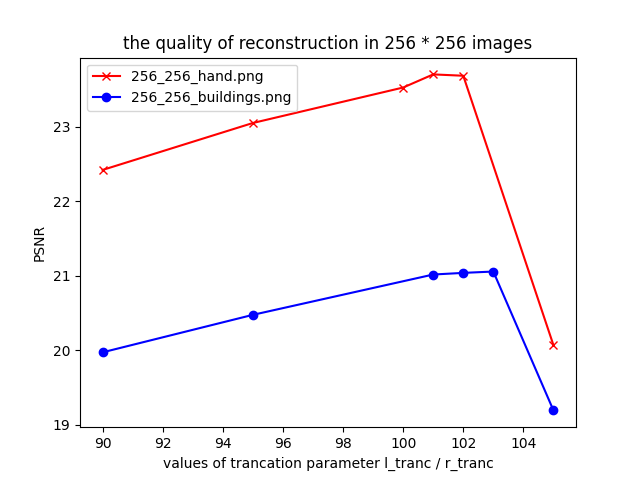
\includegraphics[width=\textwidth]{quality_256_(1).png}
    \caption{$256 \times 256$ image} 
    \label{Fig.1}
    \end{minipage}
    \begin{minipage}[t]{0.3\linewidth}
    \centering 
    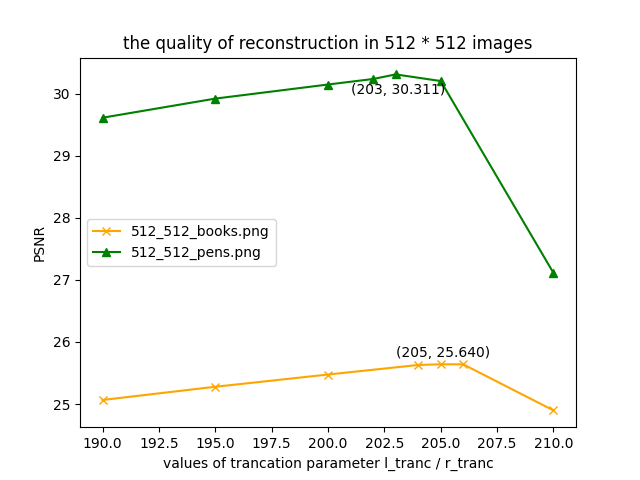
\includegraphics[width=\textwidth]{quality_512.png}
    \caption{$512 \times 512$ image}
    \label{Fig.2}
    \end{minipage}
    \begin{minipage}[t]{0.3\linewidth}
    \centering 
    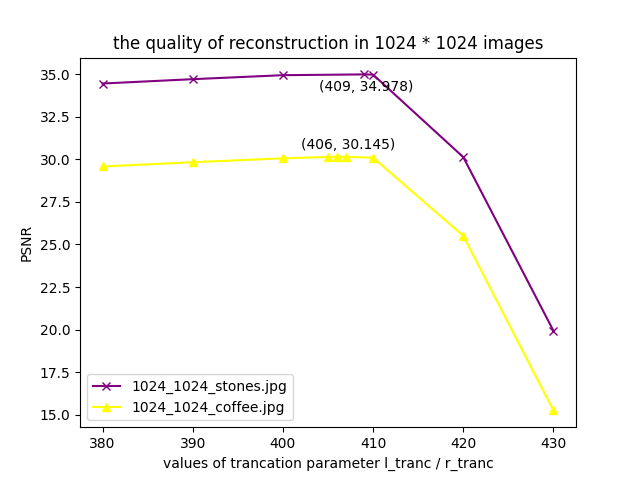
\includegraphics[width=\textwidth]{quality_1024.png}
    \caption{$1024 \times 1024$ image}
    \label{Fig.3}
    \end{minipage}
\end{figure}
The above three figures show the results obtained by applying 6 images to model I with various sizes. An observation of the relation between peak-signal-to-noise ratio (PSNR) and trancation parameters $l_{\text{trunc}}$ and $r_{\text{trunc}}$ is that the PSNR increases as the trancation parameters increase when $l_{\text{trunc}} = r_{\text{trunc}} < l^*$. When $l_{\text{trunc}} = r_{\text{trunc}} = l^*$, the reconstructed image will have the largest PSNR.  When the trancation parameters are larger than the optimal value $l^*$, the PSNR of the reconstruction sharply decreases. Another observation is that the value of the thereshold $l^*$ depends on the size of the image. From Figure 1, the trancation value which gives the best quality of reconstruction is around $102$ ($101$ for \lstinline{256_256_hand.png} and $103$ for \lstinline{256_256_buildings.png}). As for $512 \times 512$ images, the optimal value of $l_{\text{trunc}}$ and $r_{\text{trunc}}$ is around $203$. For $1024 \times 1024$ images, this value will change to around $406$.

\subsubsection{Quality of Reconstruction in Model II}
The experiment on model II presents a result that is different from model I. 
\begin{figure}[H]
    \centering
    \begin{minipage}[t]{0.45\linewidth} 
    \centering
    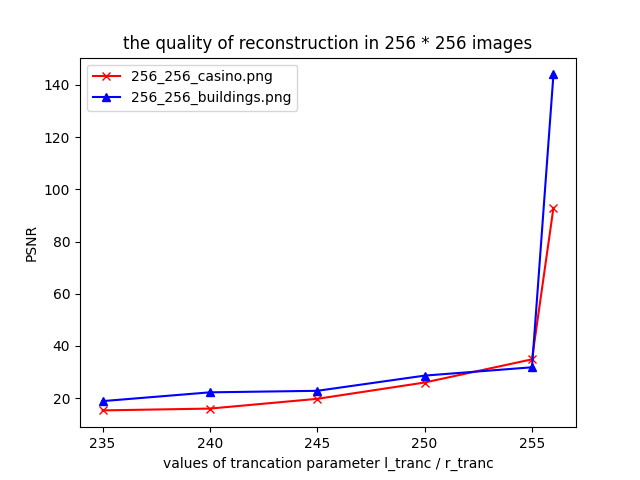
\includegraphics[width=\textwidth]{quality_256_model2.png}
    \caption{$256 \times 256$ image} 
    \end{minipage}
    \begin{minipage}[t]{0.45\linewidth}
    \centering 
    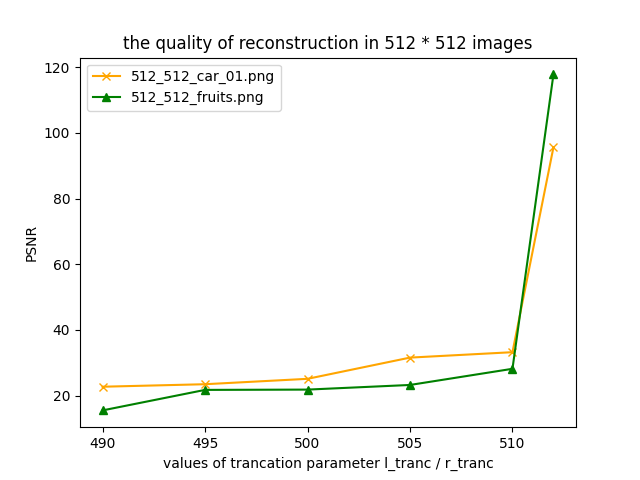
\includegraphics[width=\textwidth]{quality_512_model2.png}
    \caption{$512 \times 512$ image}
    \end{minipage}
\end{figure}
In this case, the PSNR increases as the value of the trancation parameter increases. In addition, the PSNR increases sharply when the last singular value and singular vectors are applied to construct pseudoinverse. The corresponding data and the effect of deblurring in this model are shown in Appendix-2.2.
\section{Appendix}
\subsection{Appendix-1.1: procedure of QR iteration using Wilkinson Shift and Deflation}
\begin{equation}\notag
\begin{aligned}
    &\text{input: $A \in \mathbb{R}^{n \times n}$} \\
    &\text{set $Q = Q_{\text{tmp}} = I_n \in \mathbb{R}^{n \times n}$}\\
    &\text{for $r = n$ to 2 do:}\\
    & \quad k = 0, \quad X^0 = A(1:r, 1:r) \\
    & \quad \text{while True:} \\
    & \qquad k = k + 1 \\
    & \qquad \sigma_{k - 1} = \text{Wilkinson_shift$(X^{k - 1})$}\\
    & \qquad Q_kR_k = X^{k - 1} - \sigma_{k - 1}I \\
    & \qquad X^{k} = R_kQ_k + \sigma_{k - 1}I \\
    & \qquad Q_{\text{tmp}} = Q_{\text{tmp}} \cdot Q_k \\
    & \qquad \text{if $X^k(1:r-1, r) < tol$:} \\
    & \qquad \quad \lambda_r = X^k(r, r) \\
    & \qquad \quad Q = Q \cdot \left[\begin{matrix} Q_{\text{tmp}} & \mathbf{0} \\ \mathbf{0} & I_{n - r} \end{matrix}\right] \\
    & \qquad \quad \text{break} \\
    & \lambda_1 = X^k(1, 1) \\
    & \text{end} \\
    & \text{output: $\lambda_i, \ i = 1, \cdots, n$; $Q \in \mathbb{R}^{n \times n}$} \\
\end{aligned}
\end{equation}
\subsection{Appendix-1.2: example of the output in part 1}
In this example, the following matrix $A$ is applied to the program. 
\begin{equation}\notag
    A = \left[\begin{matrix}
        17 & 21 & 31 & 45 \\
        21 & 32 & 78 & 10 \\
        9 & 15 & 2 & 62 \\
        20 & 42 & 54 & 73 \\
        38 & 25 & 2 & 19 \\
        45 & 36 & 27 & 18 \\
    \end{matrix}\right]
\end{equation}
To varify whether the QR iteration or the alternative iterative procedure give a precise result, the python inbuilt function \lstinline{numpy.linalg.svd} is used to compare with the output. 

\begin{figure}[H]
\centering
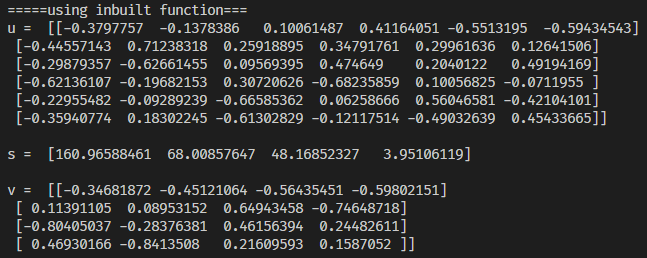
\includegraphics{Example_result_inbuilt.png}
\caption{the SVD of $A$ using python inbuilt function}
\end{figure}

\begin{figure}[H]
    \centering
    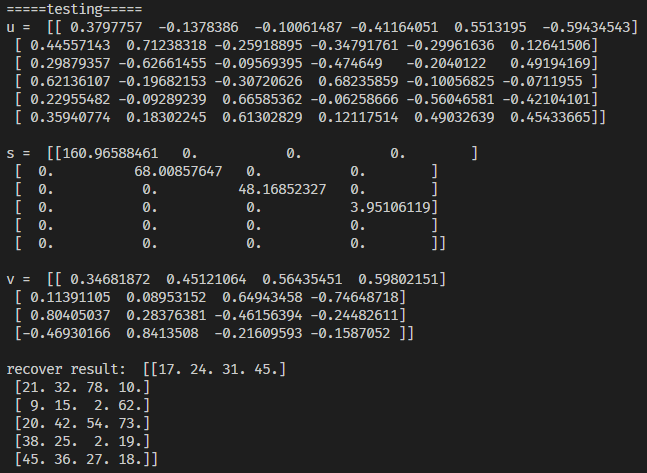
\includegraphics[height=60mm, width=100mm]{Example_result_testing.png}
    \caption{the SVD of $A$ using QR iteration with wilkinson shift and deflation}
\end{figure}

\begin{figure}[H]
    \centering
    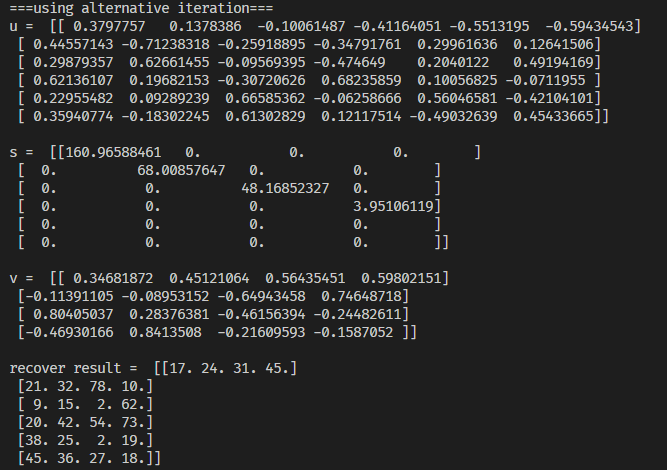
\includegraphics[height=60mm, width=100mm]{Example_result_alternative.png}
    \caption{the SVD of $A$ using alternative iterative procedure}
\end{figure}
\subsection{Appendix-2.1: examples and data obtained when measuring the quality of reconstruction in model I}
\begin{enumerate}
\item[*] $256 \times 256$ images
\begin{table}[H]
    \centering
    \begin{tabular}{|c|c|c|}
        \hline
        \textbf{image} & \textbf{trancation number} & \textbf{PSNR} \\
        \hline
        \multirow{6}{*}{256_256_hand.png} & 90 & 22.419 \\
        \cline{2-3}
        & 95 & 23.049 \\
        \cline{2-3}
        & 100 & 23.525 \\
        \cline{2-3}
        & 101 & 23.701 \\
        \cline{2-3}
        & 102 & 23.683 \\
        \cline{2-3}
        & 105 & 20.068 \\ 
        \hline
        \multirow{6}{*}{256_256_buildings.png} & 90 & 19.972 \\
        \cline{2-3}
        & 95 & 20.475 \\
        \cline{2-3}
        & 101 & 21.016 \\
        \cline{2-3}
        & 102 & 21.038 \\
        \cline{2-3}
        & 103 & 21.056 \\
        \cline{2-3}
        & 105 & 19.193 \\ 
        \hline
    \end{tabular}
\end{table}
\item[*] $512 \times 512$ images
\begin{table}[H]
    \centering
    \begin{tabular}{|c|c|c|}
        \hline
        \textbf{image} & \textbf{trancation number} & \textbf{PSNR} \\
        \hline
        \multirow{7}{*}{512_512_books.png} & 190 & 25.065 \\
        \cline{2-3}
        & 195 & 25.278 \\
        \cline{2-3}
        & 200 & 25.475 \\
        \cline{2-3}
        & 204 & 25.629 \\
        \cline{2-3}
        & 205 & 25.640 \\
        \cline{2-3}
        & 206 & 25.639 \\
        \cline{2-3} 
        & 210 & 24.897 \\
        \hline
        \multirow{7}{*}{512_512_pens.png} & 190 & 29.613 \\
        \cline{2-3}
        & 195 & 29.921 \\
        \cline{2-3}
        & 200 & 30.148 \\
        \cline{2-3}
        & 204 & 30.237 \\
        \cline{2-3}
        & 205 & 30.311 \\
        \cline{2-3}
        & 206 & 30.204 \\
        \cline{2-3} 
        & 210 & 27.112 \\
        \hline
    \end{tabular}
\end{table}
\item[*] $1024 \times 1024$ images
\begin{table}[H]
    \centering
    \begin{tabular}{|c|c|c|}
        \hline
        \textbf{image} & \textbf{trancation number} & \textbf{PSNR} \\
        \hline
        \multirow{7}{*}{1024_1024_stones.png} & 380 & 34.443 \\
        \cline{2-3}
        & 390 & 34.698 \\
        \cline{2-3}
        & 400 & 34.932 \\
        \cline{2-3}
        & 409 & 34.978 \\
        \cline{2-3}
        & 410 & 34.964 \\
        \cline{2-3}
        & 420 & 30.124 \\
        \cline{2-3} 
        & 430 & 19.935 \\
        \hline
        \multirow{9}{*}{1024_1024_coffee.png} & 380 & 29.576 \\
        \cline{2-3}
        & 390 & 29.827 \\
        \cline{2-3}
        & 400 & 30.054 \\
        \cline{2-3}
        & 405 & 30.131 \\
        \cline{2-3}
        & 406 & 30.145 \\
        \cline{2-3}
        & 407 & 30.137 \\
        \cline{2-3} 
        & 410 & 30.093 \\
        \cline{2-3}
        & 420 & 25.506 \\
        \cline{2-3}
        & 430 & 15.266 \\
        \hline
    \end{tabular}
\end{table}
\item[*] examples of blurring and deblurring an image using model I
\begin{figure}[H]
    \centering
    \subfigure[blurry image of 1024_1024_books.png]{
        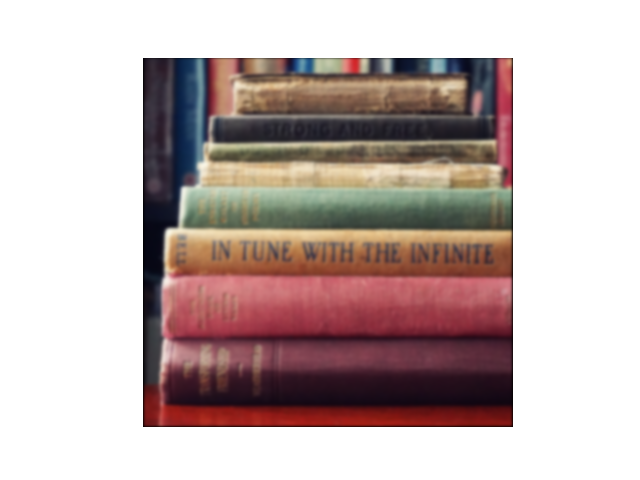
\includegraphics[width=2.75in]{blur_books_model1.png}
    }
    \subfigure[reconstruct image of 1024_1024_books.png]{
        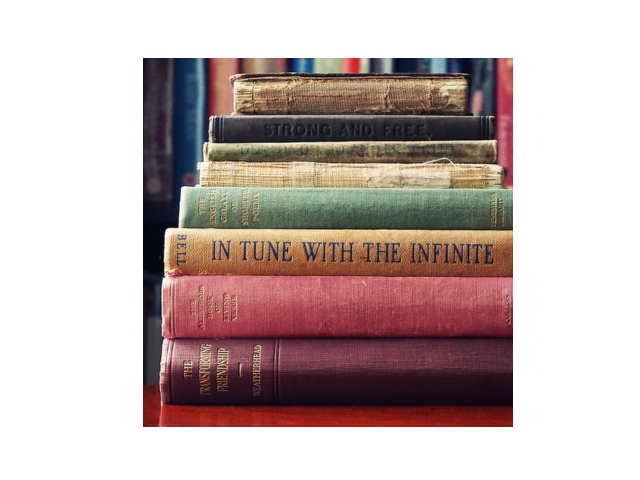
\includegraphics[width=2.75in]{reconstruct_books_model1.png}
    }
    \caption{blurry and reconstructed images of \lstinline{1024_1024_books.png} with $l_{\text{trunc}} = r_{\text{trunc}} = 406$}
\end{figure}
\begin{figure}[H]
    \centering
    \subfigure[blurry image of 512_512_fruits.png]{
        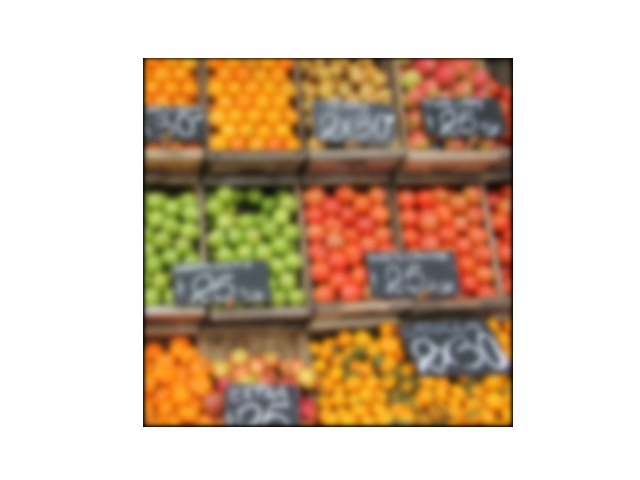
\includegraphics[width=2.75in]{blur_fruits_model1.png}
    }
    \subfigure[reconstruct image of 512_512_fruits.png]{
        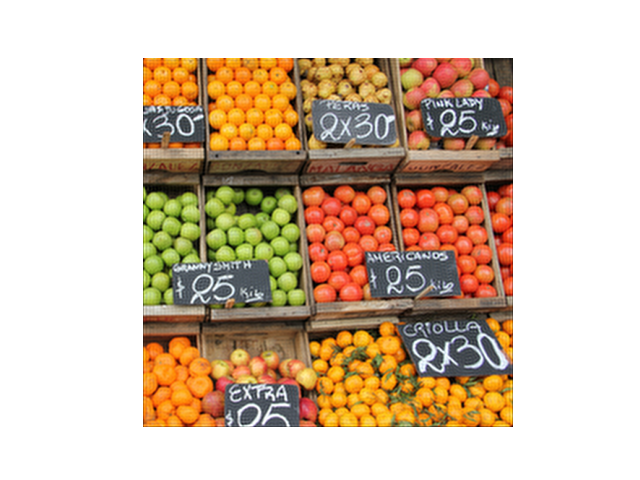
\includegraphics[width=2.75in]{reconstruct_fruits_model1.png}
    }
    \caption{blurry and reconstructed images of \lstinline{512_512_fruits.png} with $l_{\text{trunc}} = r_{\text{trunc}} = 203$}
\end{figure}
\end{enumerate}
\end{document}

% \section{Classification using NaiveBayes based on HiBench}
% 见于前

% \iffalse
% \subsection{Algorithm Description}
% Naive Bayes is a simple multiclass classification algorithm with the assumption of independence between every pair of features. It is called Naive because it assumes that the occurrence of a certain feature is independent of the occurrence of other features. It is called Bayes because it depends on the principle of Bayes' Theorem. \\

% Bayes' theorem is used to determine the probability of a hypothesis with prior knowledge. It depends on the conditional probability. The formula for Bayes' theorem is given as: P(A|B)=(P(B|A)P(A))/(P(B)). Where, P(A|B) is Posterior probability: Probability of hypothesis A on the observed event B. P(B|A) is Likelihood probability: Probability of the evidence given that the probability of a hypothesis is true. P(A) is Prior Probability: Probability of hypothesis before observing the evidence. P(B) is Marginal Probability: Probability of Evidence. Then, we have   where, y is class variable and X is a dependent feature vector (of size n). Now, we need to create a classifier model. For this, we find the probability of given set of inputs for all possible values of the class variable y and pick up the output with maximum probability. This can be expressed mathematically as: .\\

% Naive Bayes is to classify the maximum probability category.\\

% Naive Bayes classification is divided into several stages. First, generate and input training sample set, that is, all data to be classified. Second, calculate the occurrence frequency of each category in the training sample and the conditional probability estimation of each category by each characteristic attribute division, and record the results. Third, use the classifier to classify the items, and output the mapping relationship between the items to be classified and the categories and find the  maximum probability category.

% \subsection{Settings and Performance Metrics}
% In the experiment, we will explore execution time in different parameter settings, including data size, mapper number and reducer number.
% When we explore the relationship between execution time and data size, we set mapper number and reducer number to 4. When we explore the relationship between execution time and mapper number and reducer number, we set data size to tiny and set mapper number and reducer number to 1, 2 and 3 respectively, and that is 3×3=9 groups of tests.
% For data generating, we directly run the data generating script:

% sh HiBench3/bin/workloads/ml/bayes/prepare/prepare.sh

% \subsection{Experiment Data Figures/Tables}
% Run time in different data size with mapper=4 and reducer=4.\\
% \begin{center}
% \begin{tabular}{|l|l|}
%     \hline Input data size & time(s) \\
%     \hline tiny 92410458 & $371.532$ \\
%     \hline small 110928826 & $548.425$ \\
%     \hline large 373700496 & $759.175$ \\
%     \hline huge 1871682834 & $2161.719$ \\
%     \hline gigantic 3743559021 & $6181.525$ \\
%     \hline bigdata 74925678156 & $19091.845$ \\
%     \hline
% \end{tabular}
% \end{center}

% Run time in tiny data size with different mapper and reducer number.
% \begin{array}{|l|l|l|l|}
%     \hline \multirow{2}{|l|}{\text { mapper }} & 1 & 2 & 3 \\
%     \hline 1 & 390.118 & 358.760 & 351.511 \\
%     \hline 2 & 370.122 & 353.591 & 356.100 \\
%     \hline 3 & 373.230 & 343.864 & 378.076 \\
%     \hline
% \end{array}


% \fi

% \section{Matrix Multiplication}

% \subsection{Matrix Multiplication Algorithm}
% In the two Python code provided in the AIRS Cloud, one mapper and one reducer were implemented to compute the product of two matrices given by such formula:

% $$
% C=(AB)_{ij}=\sum^n_{r=1}a_{ir}b_{rj}
% $$
% For the purpose of distributed computing as a core feature of MapReduce, the computation process should be separated into independent procedures so that computation might be done on various nodes. By the formula above, we learn that $c_{ij}$ are independent from each other, so that we can put them into the same key in the map phase. Then, in the reduce stage we can compute $C$ by analyzing different elements. 

% \subsection{Matrix Multiplication in MapReduce}
% MapReduce is a programming model developed by Google and made available as an Apache open source project . The model is used for processing large data sets across clusters of computers using a shared filesystem. Specifically, it is implemented in a fashion where user programs only need to ' Map' input data to values stored in a global distributed file system, and ' Reduce' those values to derive the final output . Because of its origins, its terms tend to reflect that origin with code that is written in Java and Python. 

% In our experiment, we first uploaded the input files to Hadoop’s HDFS file system:

% \lstset{language=command.com}
% \begin{lstlisting}
%     hadoop fs -put /home/team18/matrix/L1.txt /dataspace/team18/matrix/L1.txt
%     hadoop fs -put /home/team18/matrix/R1.txt /dataspace/team18/matrix/R1.txt
% \end{lstlisting}

% Then we gave writing and reading access to them:

% \begin{lstlisting}
%     hadoop fs -chmod 777 /dataspace/team18/matrix/
% \end{lstlisting}

% Once the input files are uploaded and accessible through the HDFS file system, we began using Hadoop’s streaming utility:

% \begin{lstlisting}
%     mapred streaming -input /dataspace/team18/matrix \
% 	-file /home/team18/matrix/MatMulMapper.py \
% 	-mapper "python MatMulMapper.py" \
% 	-file /home/team18/matrix/MatMulReducer.py \
% 	-reducer "python MatMulReducer.py" \
% 	-output /dataspace/team18/matrix-output
% \end{lstlisting}

% Which yields the results as follows:

% \begin{lstlisting}
%     22/11/28 08:47:35 INFO mapreduce.Job: The url to track the job: http://master2.cuhk.com:8088/proxy/application_1669595859297_0007/
%     22/11/28 08:47:35 INFO mapreduce.Job: Running job: job_1669595859297_0007
%     22/11/28 08:47:42 INFO mapreduce.Job: Job job_1669595859297_0007 running in uber mode : false
%     22/11/28 08:47:42 INFO mapreduce.Job:  map 0% reduce 0%
%     22/11/28 08:47:50 INFO mapreduce.Job:  map 100% reduce 0%
%     22/11/28 08:48:02 INFO mapreduce.Job:  map 100% reduce 100%
%     22/11/28 08:48:36 INFO mapreduce.Job: Job job_1669595859297_0007 completed successfully
%     22/11/28 08:48:36 INFO mapreduce.Job: Counters: 53
%         File System Counters
%             FILE: Number of bytes read=184842966
%             FILE: Number of bytes written=370439648
%             FILE: Number of read operations=0
%             FILE: Number of large read operations=0
%             FILE: Number of write operations=0
%             HDFS: Number of bytes read=23083042
%             HDFS: Number of bytes written=393911
%             HDFS: Number of read operations=11
%             HDFS: Number of large read operations=0
%             HDFS: Number of write operations=2
%         Job Counters
%             Launched map tasks=2
%             Launched reduce tasks=1
%             Data-local map tasks=2
%             Total time spent by all maps in occupied slots (ms)=34152
%             Total time spent by all reduces in occupied slots (ms)=264864
%             Total time spent by all map tasks (ms)=11384
%             Total time spent by all reduce tasks (ms)=44144
%             Total vcore-milliseconds taken by all map tasks=11384
%             Total vcore-milliseconds taken by all reduce tasks=44144
%             Total megabyte-milliseconds taken by all map tasks=34971648
%             Total megabyte-milliseconds taken by all reduce tasks=271220736
%         Map-Reduce Framework
%             Map input records=2048
%             Map output records=16384
%             Map output bytes=184777424
%             Map output materialized bytes=184842972
%             Input split bytes=202
%             Combine input records=0
%             Combine output records=0
%             Reduce input groups=72
%             Reduce shuffle bytes=184842972
%             Reduce input records=16384
%             Reduce output records=16448
%             Spilled Records=32768
%             Shuffled Maps =2
%             Failed Shuffles=0
%             Merged Map outputs=2
%             GC time elapsed (ms)=759
%             CPU time spent (ms)=51570
%             Physical memory (bytes) snapshot=2747916288
%             Virtual memory (bytes) snapshot=16727359488
%             Total committed heap usage (bytes)=2665480192
%             Peak Map Physical memory (bytes)=2122207232
%             Peak Map Virtual memory (bytes)=4675809280
%             Peak Reduce Physical memory (bytes)=1531682816
%             Peak Reduce Virtual memory (bytes)=8512802816
%         Shuffle Errors
%             BAD_ID=0
%             CONNECTION=0
%             IO_ERROR=0
%             WRONG_LENGTH=0
%             WRONG_MAP=0
%             WRONG_REDUCE=0
%         File Input Format Counters
%             Bytes Read=23082840
%         File Output Format Counters
%             Bytes Written=393911
%     22/11/28 08:48:36 INFO streaming.StreamJob: Output directory: /dataspace/team18/matrix-output-8
% \end{lstlisting}

% After the MapReduce is successfully done on the remote machine, we then run the clean up command to delete the generated output directory after copying the result to local file system. 

% To experiment further, we used the pipe operator to run the mapper and reducer separately locally to make sure the functions work correctly: 

% \lstset{language=C++}
% \begin{lstlisting}
%     cat L1.txt, R1.txt | python3 MatMulMapper.py | python3 MatMulReducer.py
% \end{lstlisting}

% Now in the application of the MapReduce algorithm to the matrix multiplication problem, we studied the following aspects. 

% First is the data or file structure. Matrix data is stored in binary and separated by lines. The former led to the use of the `binascii` module and the latter is to make separation of concerns easier done. 

% Second is the computation process. To convert the algorithm into MapReduce, we have to implement three phases: map, shuffle and reduce. 

% In the map phase, we marke $a_{ij}$ to `<key, value>` of number I, where `key` = $(i,k), k =1,2,...I$ and `value` = $(a, j, a_{ij}).$ The same goes for the $B$ matrix. The key bridges the computation results, and the value separates numbers from different matrices. 

% \lstset{language=Python}
% \begin{lstlisting}
%     if A_B == "L":
%     ib = (int)(lineno)/BLOCKSIZE  # note here the input data starts from 1, the result may differ from that in ppt
%     for jb in range(NB):
%         # the key is the BLOCK Number
%         intermediate_key = '%05d'%(ib * NB + jb)
%         # the value is the {L/R}:{LineNo}:{values of current line}
%         intermediate_value = 'L:%s:%s'%(lineno, row_value)
%         # key and value are seperated by a tab
%         print("%s\t%s" % (intermediate_key, intermediate_value))

% if A_B == "R":
%     jb = (int)(lineno)/BLOCKSIZE
%     for ib in range(NB):
%         intermediate_key = '%05d'%(ib * NB + jb)
%         intermediate_value = 'R:%s:%s'%(lineno, row_value)
%         print("%s\t%s"%(intermediate_key, intermediate_value))
% \end{lstlisting}

% In the shuffle phase, values with the same key will be packed into a list and passed to reduce. This is automatically done by Hadoop. 

% In the reduce phase, we have constructed the key as a form in the Map stage. And we also marked in the Map phase. The next thing to do is to parse the list(value), the elements from are placed in an array alone, and the elements from are placed in another array. Then, we calculate two arrays (each as a vector ), the value that can be calculated.

% \lstset{language=Python}
% \begin{lstlisting}
%     blockno = int(input_key)
%     A_B, index, row_value = input_value.split(":")

%     if A_B == "L":
%         LeftMatrixBlock.append(row_value.split(" "))
%     if A_B == "R":
%         RightTransposeMatrixBlock.append(row_value.split(" "))

% res = [[0 for col in range(BLOCKSZIE)] for row in range(BLOCKSZIE)]
% for i in range(BLOCKSZIE):
%     for j in range(BLOCKSZIE):
%         for k in range(TOTALSIZE):
%             left_val = int(struct.unpack("I", binascii.a2b_hex(LeftMatrixBlock[i][k][2:]))[0])
%             right_val = int(struct.unpack("I", binascii.a2b_hex(RightTransposeMatrixBlock[j][k][2:]))[0])
%             res[i][j] += left_val * right_val
%         print(res[i][j])
% \end{lstlisting}

% \section{Image Classification}
% \subsection{The structure of network structure}
% % \begin{figure}[H]
% %     \centering
% %     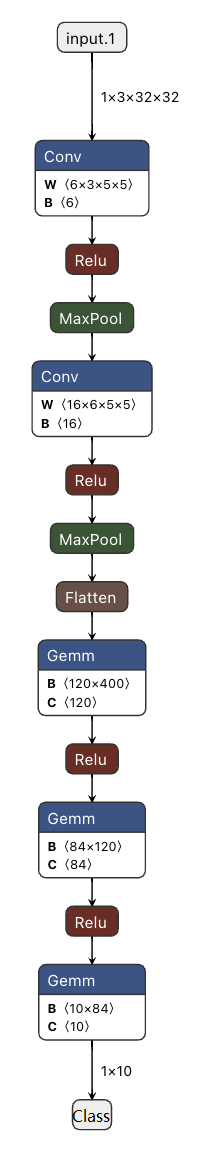
\includegraphics[width=4cm]{微信图片_20221127145950.png}
% %     \end{figure}
% In this report, we use CNN to classify the images, where Conv get the feature of the input and Relu to activate and then use pool to up sampling. This CNN is Feedforward neural network.

% \subsection{Result with default settings}
% The training loss with default settings are below.
% % \begin{figure}[H]
% %     \centering
% %     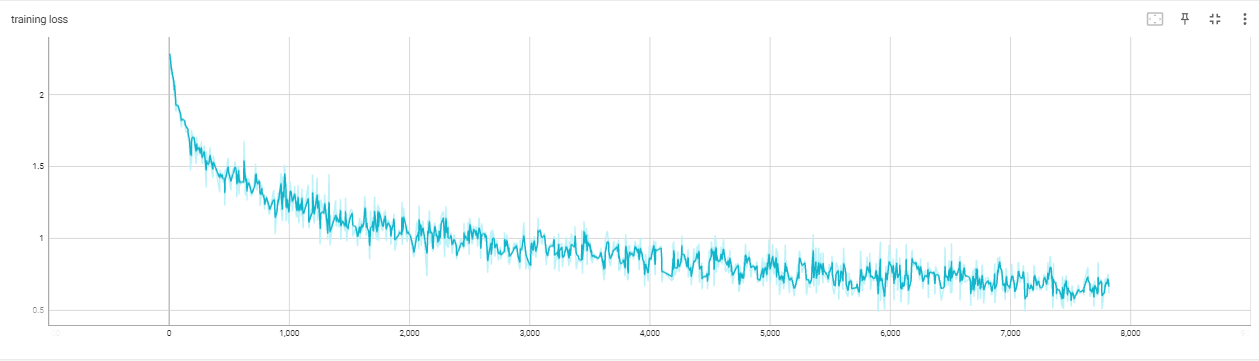
\includegraphics[width=16cm]{Pasted image 20221127162033.png}
% % \end{figure}

% The accuracy with default settings are below.(where X-axis is time)
% % \begin{figure}[H]
% %     \centering
% %     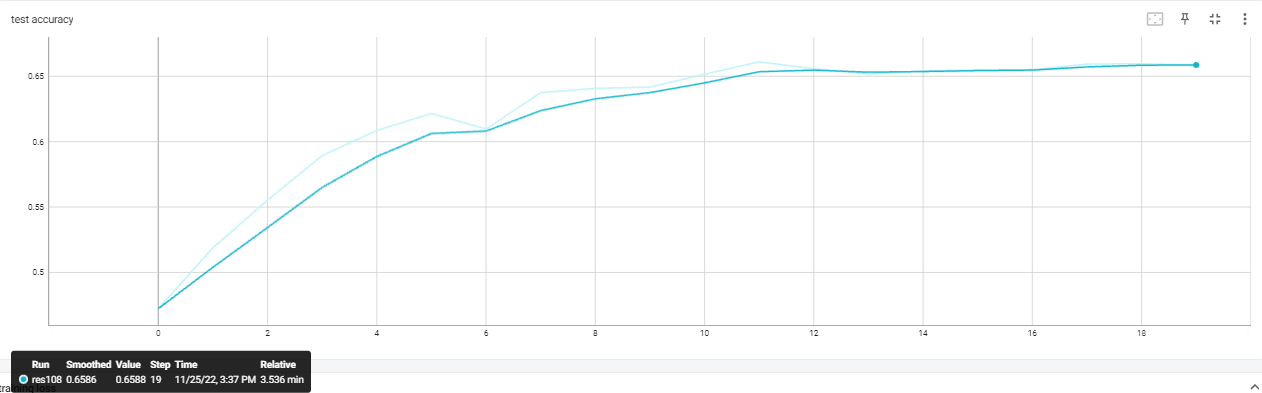
\includegraphics[width=16cm]{Pasted image 20221127161956.png}
% % \end{figure}

% With the training, the accuracy trend to be 66\%. training time are 3.536mins.

% \subsection{Result with different settings}

% \textbf{In this section, we use different settings to obtain the task, and the result are below.}
% % \begin{figure}[H]
% %     \centering
% %     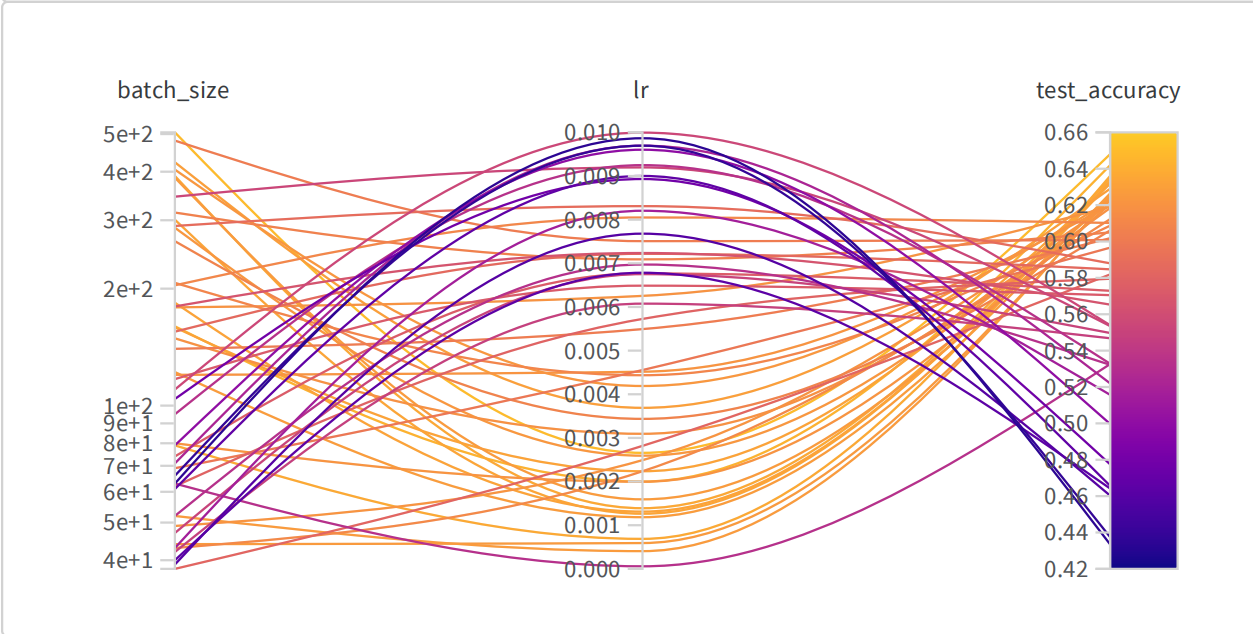
\includegraphics[width=16cm]{Pasted image 20221127160754.png}
% % \end{figure}
% Through the picture, we can see the best accuracy is obtained with batch size = 4e+2 and the learning rate =0.002.\\
% However, with other model, we get a higher acc.\\
% The baseline is 63\% (blue line),using 3 mins.\\
% When we use resnet108, we can get an acc about 81\%(black line), using 30 mins.\\
% With Vit_small, we get an acc about 82\%(purple line), using 36mins.\\
% With swinv2, we get an acc about 98\%(yellow line), using1.21 hrs.\\
% % \begin{figure}[H]
% %     \centering
% %     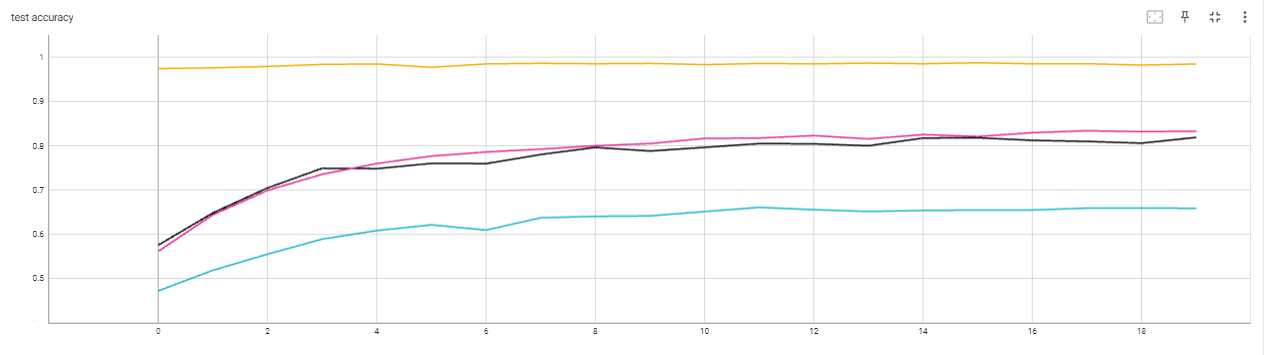
\includegraphics[width=16cm]{Pasted image 20221127162523.png}
% % \end{figure}

% % \subsection{Recording of system run time information
% % }

% % The CPU usage is below.
% % \begin{figure}[H]
% %     \centering
% %     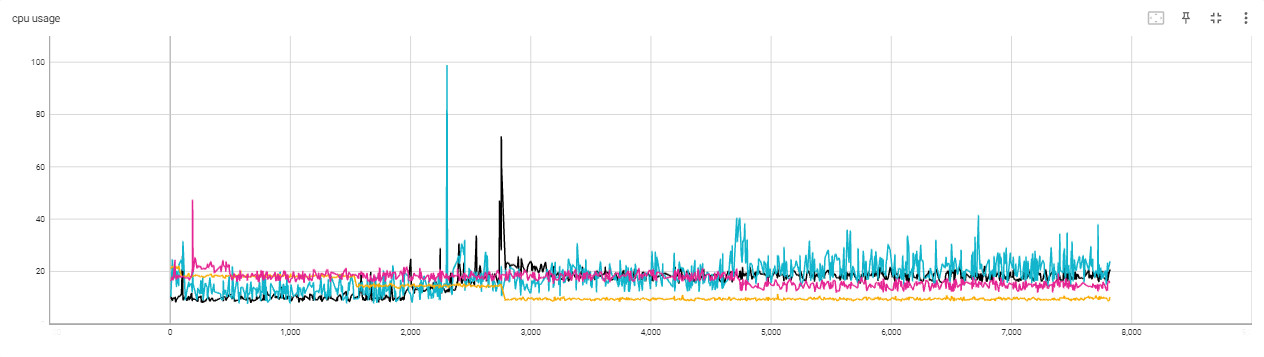
\includegraphics[width=16cm]{Pasted image 20221127163308.png}
% % \end{figure}

% % The GPU usage is below.
% % \begin{figure}[H]
% %     \centering
% %     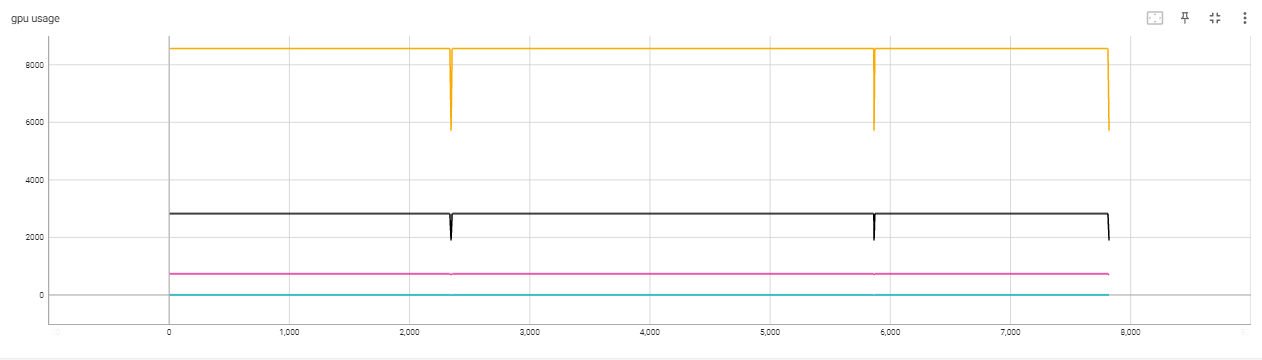
\includegraphics[width=16cm]{Pasted image 20221127163454.png}
% % \end{figure}

% The baseline is blue line, the resnet108 is black line, Vit_small is purple line and the swinv2 is yellow line.\\
% Through the usage of system, we can see the usage of CNN provided is low at first. Then it increases and waves frequently. It may be the simple structure of the network and the thread of CPU. And the usage of GPU is constant, which is mainly because the parallel computing of GPU is high.

% \section{Image to Text}
% \subsection{Experiment Specification}
% The experiment background is a image captioning task on the dataset COCO2014 (Microsoft Common Objects in Context) 
% invloving Computer Vision and Natural Language Processing. Rather than performing large-scale object detection, segmentation, key-point detection, and captioning, which COCO2014
% is commonly adopts, our model only performs the captioning, i.e, for an input image , the model outputs the caption of objects in the image.\\
% Our experiment is to train the model with different hyperparameters and compare the model performance under different metrics. We are tuning the following hyperparameters: 
% $batch\_size$ \\
% Encoder (Convolutional Neural Network): $embed\_size$\\
% Decoder (Recurrent Neural Network): $embed\_size$, $num\_layers$, $hidden\_size$\\
% Optimizer (Adam): $learning\_rate$

% \subsection{Interpretation of Perplexity}
% Perplexity is a common performance metric in NLP. Concisely, Perplexity is the exponential of Cross-Entropy. For a given sentence 
% $W = (w_{1}, w_2, \cdots, w_n)$, where $w_{i}$ denotes the $i$th word, its Perplexity is defined as:
% \begin{equation}
%     Perplexity(W) = 2^{H(W)}
% \end{equation}
% where $H(W)$ denotes the Cross-Entropy of $W$, noted that the base is not necessarily be 2, in our experiment, we use $e$.
% Entropy denotes the expectation of information, after simplifying we get
% \begin{equation}
%     H(W) = -\log{P(w_{1}, w_2, \cdots, w_n)}
% \end{equation}
% In the view of bit-length, Perplexity can be interpreted as the number of outputs that are of the same probability (that's why we commonly use 2 as the base in Eq.1). 
% For a given historical information, the less equal probability outputs, the less 'confused' the model is and hence the better modeling. 

% \subsection{Analysis of Different Hyperparameters}
% Notice that while we try different hyperparameters, we do it in a control experiment manner and keep other hyperparameters of their default 
% setting:\\
% \begin{table}[!ht]
% \caption{Default Setting}
% \centering
% \begin{tabular}{|c|c|c|c|c|}\hline
%    $embed\_size$ & $num\_layers$ & $batch\_size$ & $hidden\_size$ & $learning\_rate$ \\ \hline
%     299&1&128&512&0.001 \\ \hline
% \end{tabular}
% \end{table}
% \subsubsection{embed\_size}
% $embed\_size$ is a hyperparameter shared by both encoder and decoder. Generally, large $embed\_size$ will not hurt the model performance but
% results in higher training cost. We tried $embed\_size = \{50,100,200,300,400\}$, the performance and time cost for each $embed\_size$:\\
% % \begin{figure}[H]
% %     \centering 
% %     \begin{minipage}[b]{0.3\textwidth} 
% %     \centering 
% %     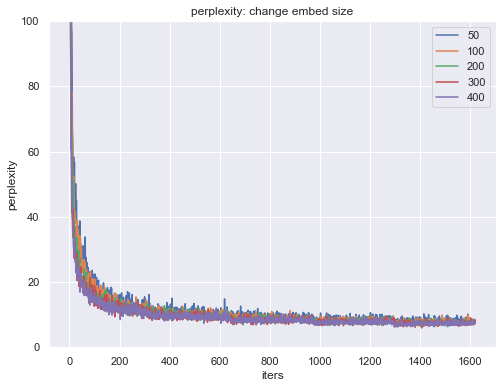
\includegraphics[width=0.9\textwidth]{p_embedsize.png}
% %     \caption{Perplexity} 
% %     \label{Fig.1}
% %     \end{minipage}
% %     \begin{minipage}[b]{0.3\textwidth}
% %     \centering 
% %     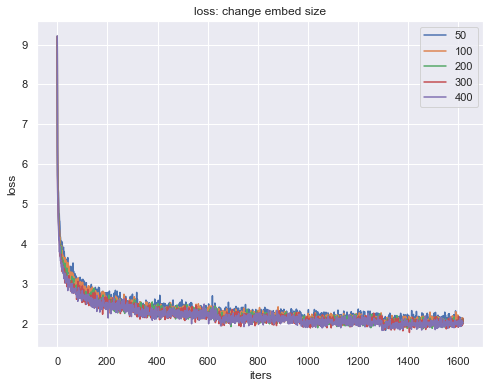
\includegraphics[width=0.9\textwidth]{l_embedsize.png}
% %     \caption{Loss}
% %     \label{Fig.2}
% %     \end{minipage}
% %     \begin{minipage}[b]{0.3\textwidth}
% %     \centering 
% %     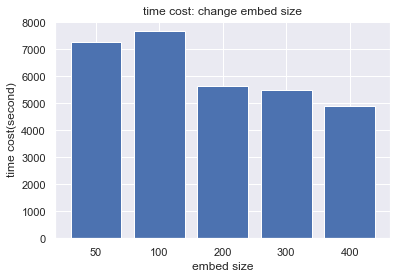
\includegraphics[width=0.9\textwidth]{time_embedsize.png}
% %     \caption{Time cost}
% %     \label{Fig.3}
% %     \end{minipage}
% % \end{figure}
% Hence we can see that $embed\_size = 400$ achieves the better accuracy and convengence speed.


% \subsubsection{learning rate}
% $learning\_rate$ is a hyperparameter in the Optimizer Adam. We tried $learning\_rate = \{0.1, 0.01, 0.001\}$, the performance and time cost for each $learning\_rate$ :
% % \begin{figure}[H]
% %     \centering 
% %     \begin{minipage}[b]{0.3\textwidth} 
% %     \centering 
% %     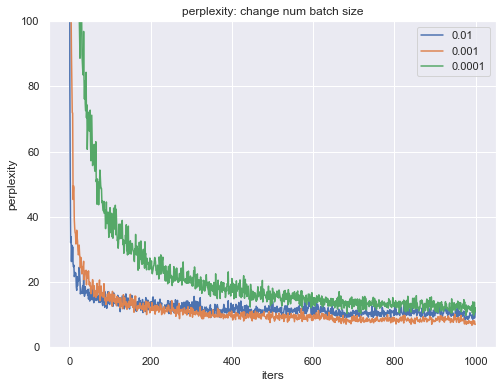
\includegraphics[width=0.9\textwidth]{p_learningrate.png}
% %     \caption{Perplexity} 
% %     \label{Fig.1}
% %     \end{minipage}
% %     \begin{minipage}[b]{0.3\textwidth}
% %     \centering 
% %     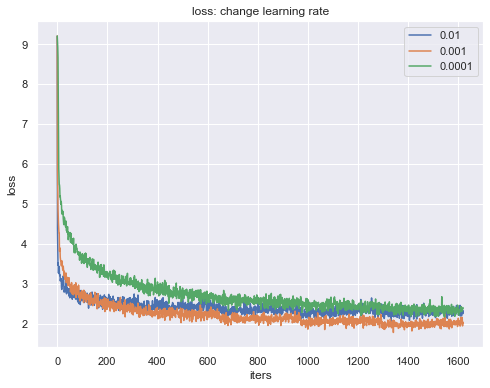
\includegraphics[width=0.9\textwidth]{l_learningrate.png}
% %     \caption{Loss}
% %     \label{Fig.2}
% %     \end{minipage}
% %     \begin{minipage}[b]{0.3\textwidth}
% %     \centering 
% %     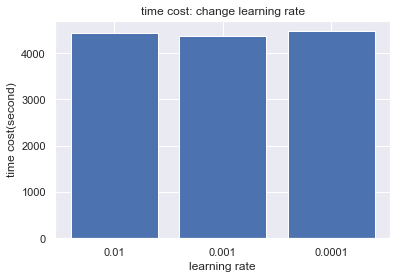
\includegraphics[width=0.9\textwidth]{time_learningrate.png}
% %     \caption{Time cost}
% %     \label{Fig.2}
% %     \end{minipage}
% % \end{figure}
% With no significant difference in time costing, a bolder choice of $learning\_rate = 0.01$ received the better Perplexity.

% \subsubsection{number of layers}
% $num\_layer$ is a hyperparameter in Decoder(LSTM). We tried $num\_layers = \{1,2,4\}$, the performance and time cost for each $num\_layer$:\\:
% % \begin{figure}[H]
% %     \centering 
% %     \begin{minipage}[b]{0.3\textwidth} 
% %     \centering 
% %     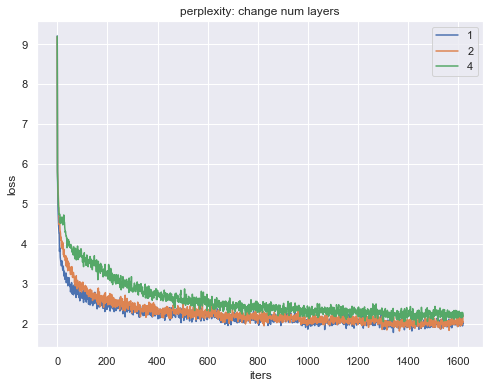
\includegraphics[width=0.9\textwidth]{p_layer.png}
% %     \caption{Perplexity} 
% %     \label{Fig.1}
% %     \end{minipage}
% %     \begin{minipage}[b]{0.3\textwidth}
% %     \centering 
% %     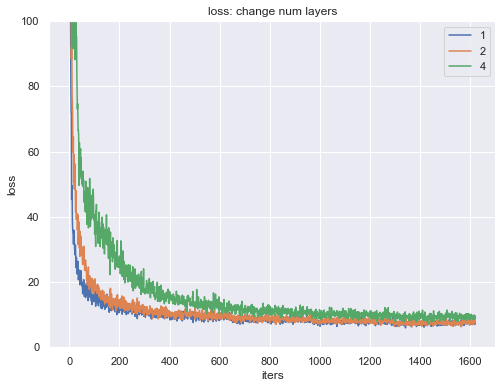
\includegraphics[width=0.9\textwidth]{l_layer.png}
% %     \caption{Loss}
% %     \label{Fig.2}
% %     \end{minipage}
% %     \begin{minipage}[b]{0.3\textwidth}
% %     \centering 
% %     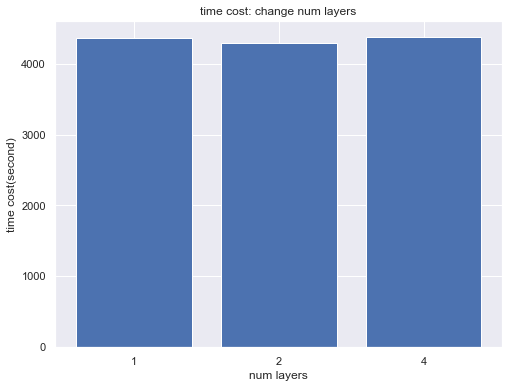
\includegraphics[width=0.9\textwidth]{time_layer.png}
% %     \caption{Time cost}
% %     \label{Fig.2}
% %     \end{minipage}
% % \end{figure}
% With no significant difference in time costing, decreasing LSTM complexity $num\_layers = 1$ received the better Perplexity and convengence speed.
% \subsubsection{hidden size}
% $hidden\_size$ is a hyperparameter in Decoder(LSTM). We tried $hidden\_size = \{128, 256, 512\}$, the performance and time cost for each $hidden\_size$:\\

% % \begin{figure}[H]
% %     \centering 
% %     \begin{minipage}[b]{0.3\textwidth} 
% %     \centering 
% %     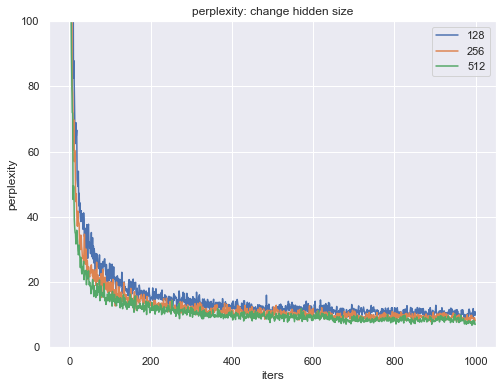
\includegraphics[width=0.9\textwidth]{p_hiddensize.png}
% %     \caption{Perplexity} 
% %     \label{Fig.1}
% %     \end{minipage}
% %     \begin{minipage}[b]{0.3\textwidth}
% %     \centering 
% %     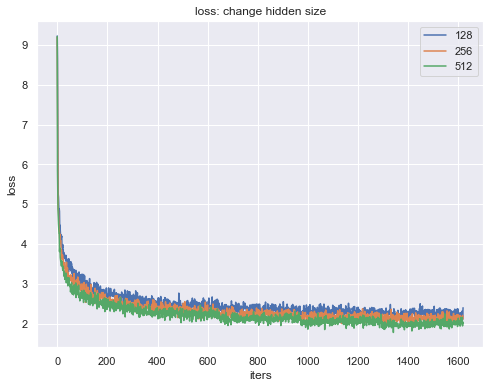
\includegraphics[width=0.9\textwidth]{l_hiddensize.png}
% %     \caption{Loss}
% %     \label{Fig.2}
% %     \end{minipage}
% %     \begin{minipage}[b]{0.3\textwidth}
% %     \centering 
% %     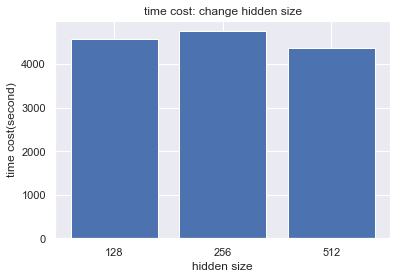
\includegraphics[width=0.9\textwidth]{time_hiddensize.png}
% %     \caption{Time cost}
% %     \label{Fig.2}
% %     \end{minipage}
% % \end{figure}
% With slightly lower time costing, increasing LSTM complexity $hidden\_sizes = 512$ received the better Perplexity and convengence speed.

% \subsubsection{batch size}
% $batch\_size$ is a hyperparameter in training. Dividing data into batches can decrease training memory usage and by updating parameters after every batch, the algorithm converges faster. The performance and time cost for each $hidden\_size$:\\
% % \begin{figure}[H]
% %     \centering 
% %     \begin{minipage}[b]{0.3\textwidth} 
% %     \centering 
% %     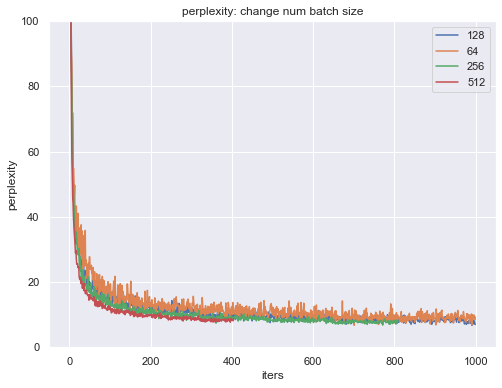
\includegraphics[width=0.9\textwidth]{p_batch.png}
% %     \caption{Perplexity} 
% %     \label{Fig.1}
% %     \end{minipage}
% %     \begin{minipage}[b]{0.3\textwidth}
% %     \centering 
% %     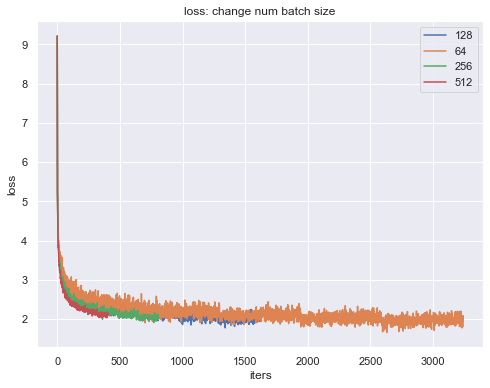
\includegraphics[width=0.9\textwidth]{l_batch.png}
% %     \caption{Loss}
% %     \label{Fig.2}
% %     \end{minipage}
% %     \begin{minipage}[b]{0.3\textwidth}
% %     \centering 
% %     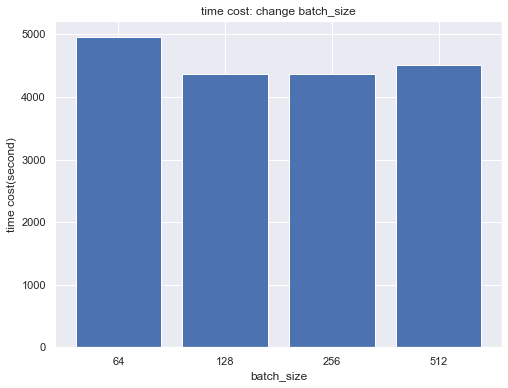
\includegraphics[width=0.9\textwidth]{time_batch.png}
% %     \caption{Time cost}
% %     \label{Fig.2}
% %     \end{minipage}
% % \end{figure}
% Dividing the training set into batches of 128 or 256 or 512 increases the training speed while $batch\_size = 512$ converges faster than others.
% \subsubsection{GPU and CPU usage analysis}
% With the increase of $batch\_size$, the use rate of CPU and GPU will both increase. That's because we need to load more data into CPU and GPU in one batch.\\
% With the increase of $learning\_rate$, the use rate of CPU and GPU will stay almost the same. That's because the learning rate have no influnce on the memory.\\
% With the increase of $hidden\_size$, the use rate of CPU stays the same. but GPU will increase because the we
% need to load more parameters to GPU.\\
% With the increase of $embed\_size$ the use rate of CPU and GPU will both increase. That's because the smaller the embed sizethe smallerthe size ofinput data, which also means smaller usage of CPU and GPU.\\
% \end{document}

% \end{document}
